\subsection{Result and Analysis}

\begin{figure}[h]
    \centering
    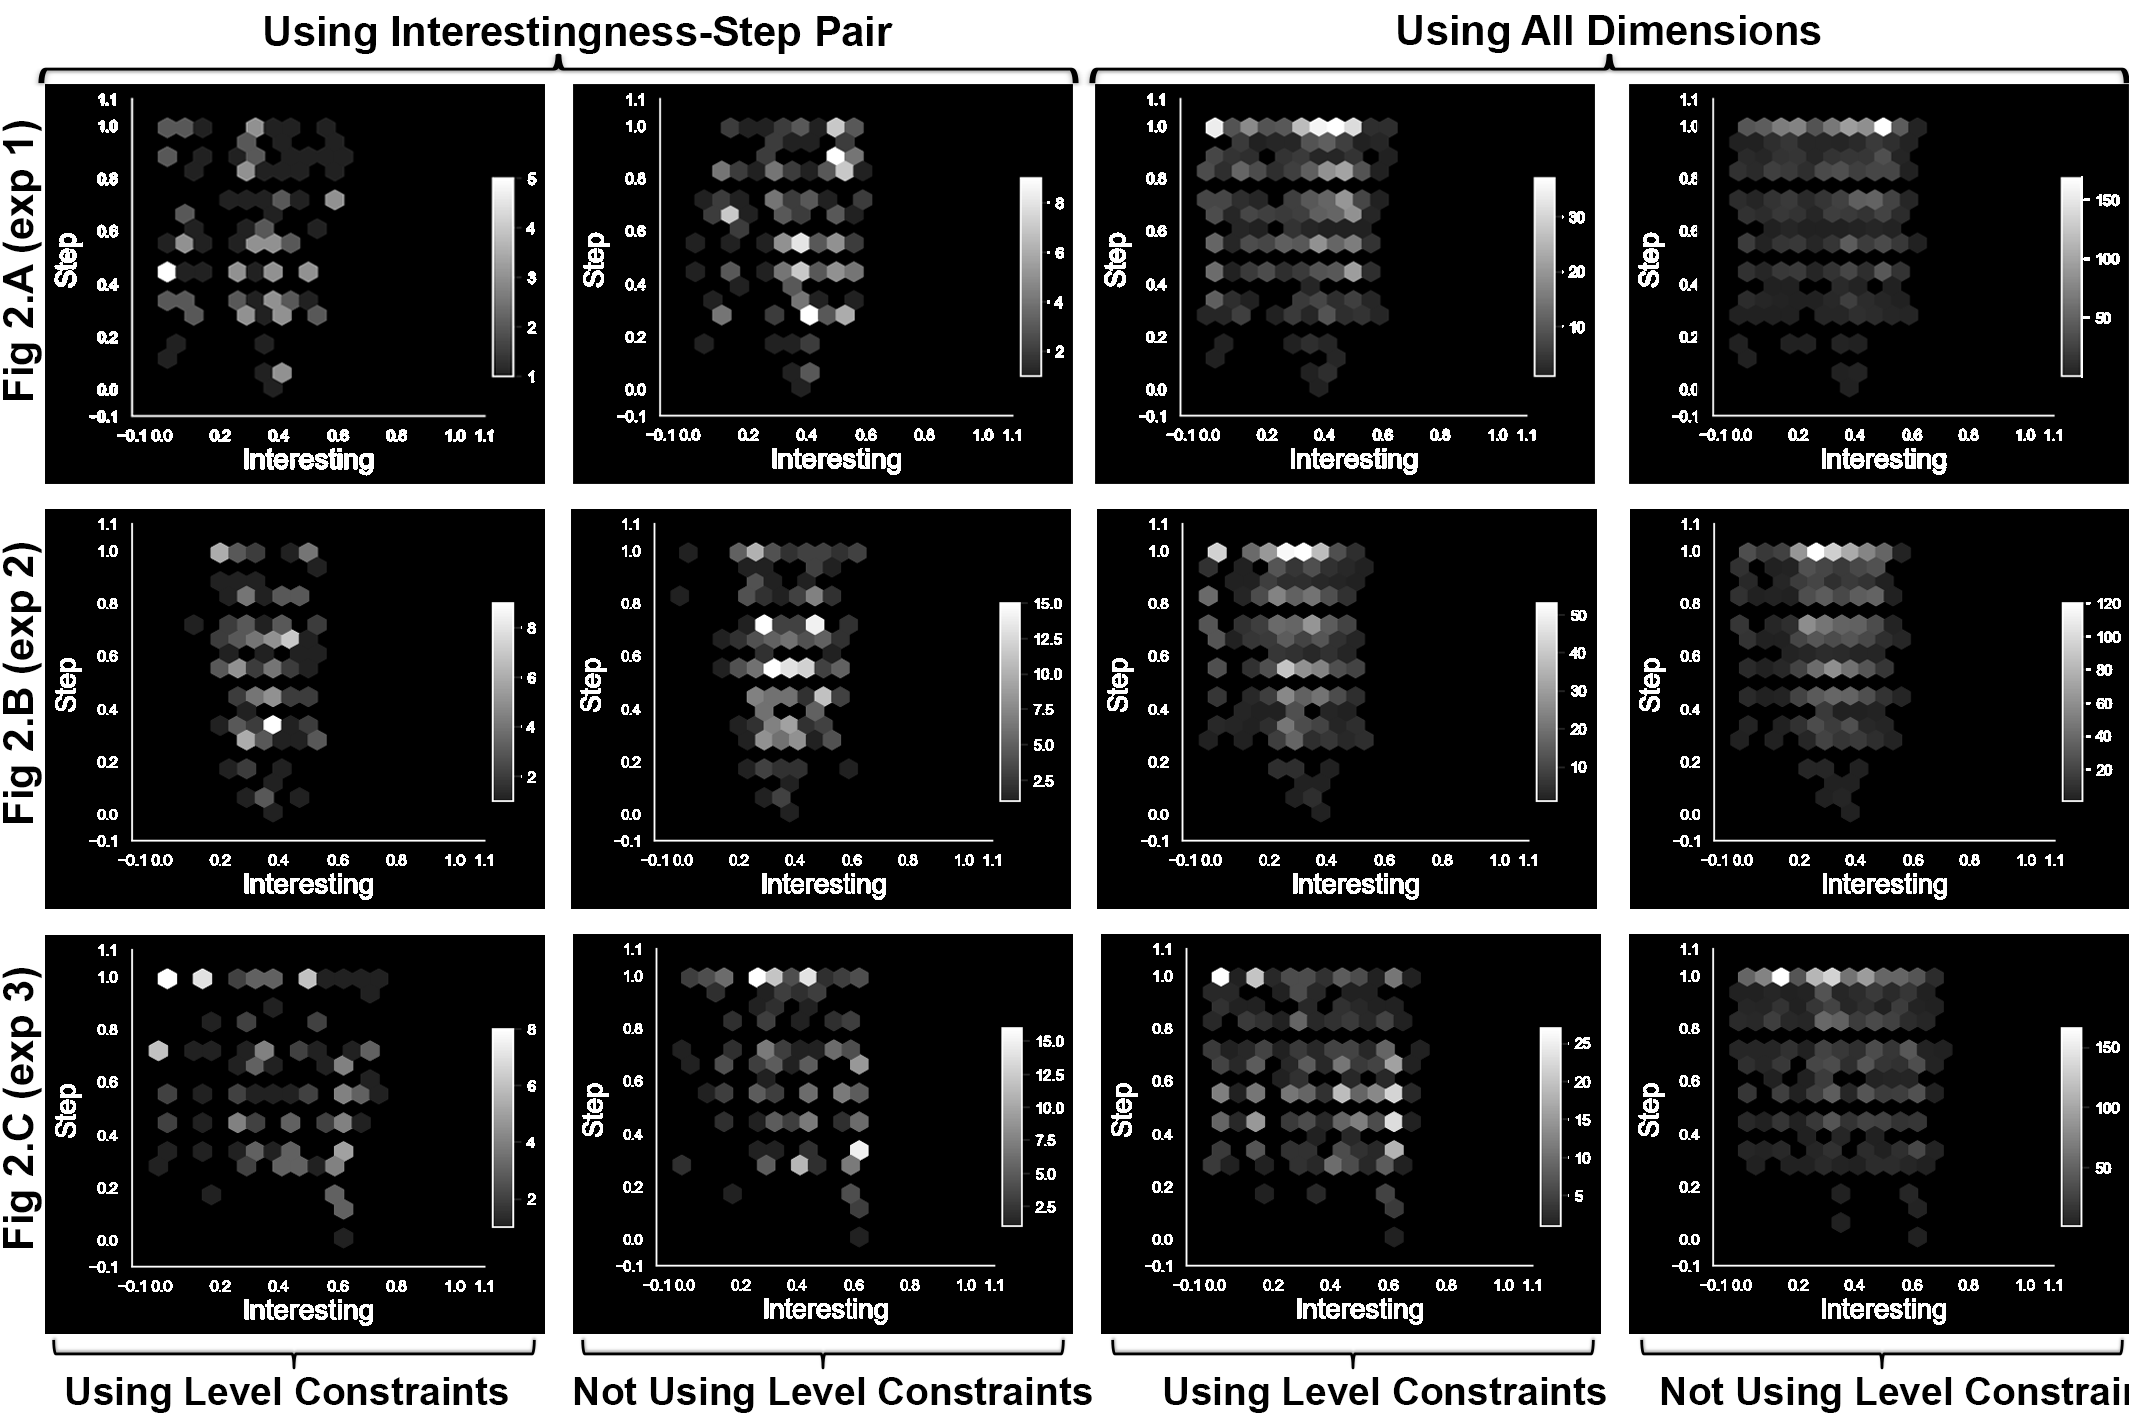
\includegraphics[width=\linewidth]{figures/experiment-123_fixed.png}
    \caption{Rows show experiment 1-3, respectively. Each narrative graph can be seen in figure~\ref{fig:examples}.a-c, respectively. The first two columns are using interestingness-step as dimensions, and the other columns are using all dimensions in the search.}
    \label{fig:experiment123}
\end{figure}

\begin{figure}[t!]
    \centering
    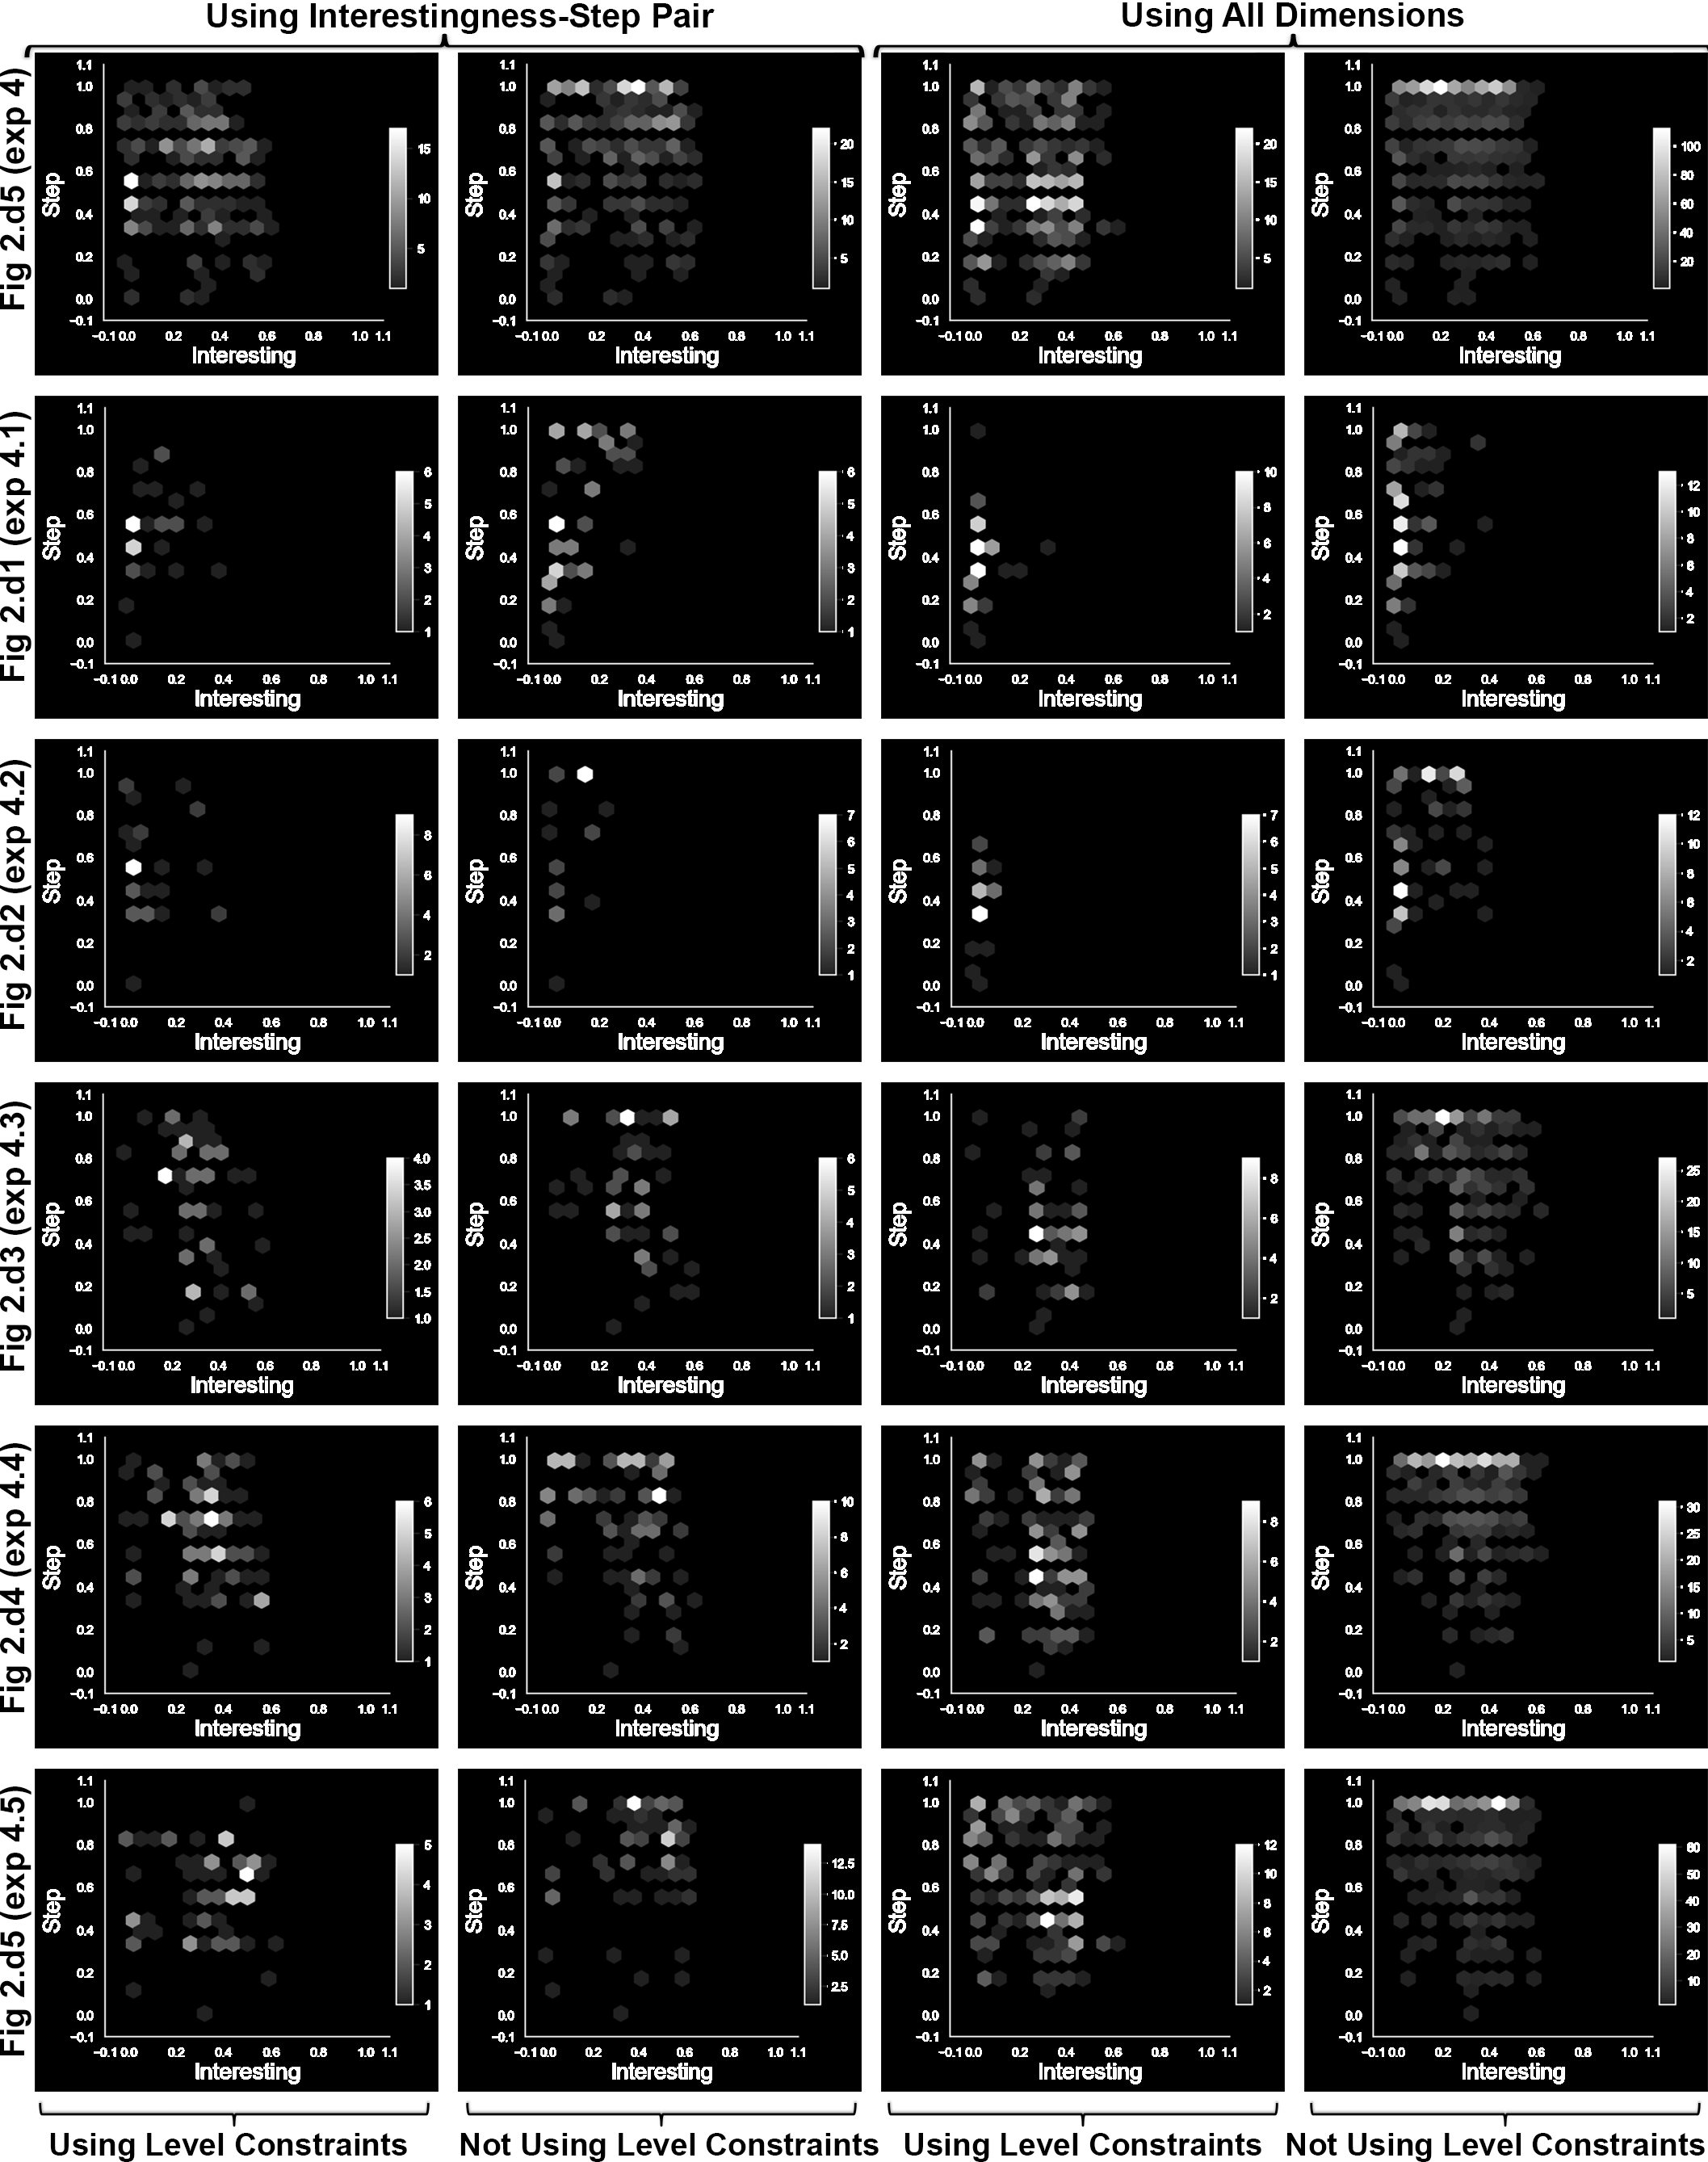
\includegraphics[width=\linewidth]{figures/experiment-4_fixed.png}
    \caption{Expressive Range Analysis (ERA) and Temporal ERA (TERA) for Experiment 4. The first row is the general results for experiment 4 (ERA), while the subsequent ones are the individual results per step taken in the narrative structure design (figure~\ref{fig:examples}.d) (TERA). The first two columns are using interestingness-step as dimensions, and the other columns are using all dimensions in the search. }
    \label{fig:experiment-stepstep}
\end{figure}

%Odd columns are with level constraints and even columns without constraints.

% \begin{itemize}
%     \item Figure with expressive range analysis (just a few of dimensions) Using different graphs \checkmark
%     \item Figure with a few generated examples! and the grid! 
%     \item Figure using constraints and not, discuss the ERA based on that. \checkmark
%     \item a table! \checkmark
%     \item Comparison within studies (pair and all dims) individually. Exp 1-4 and EXP 4.x.
%     \item Comparison within Study: Constraints vs. No constraints (Pair and all dims) individually. Exp 1-4 and EXP 4.x.
%     \item Comparison between studies: Exp 1-4 and exp 4.x.
%     \item *I Would also like to do a bit of qualitative analysis based on what is generated! 
% \end{itemize}

%\begin{table}[]
\caption{displaying the grammatical rules. The columns marked with asterisks are identified as “motivations” by Doran and Parberry~\cite{Doran2011-questsMMORPGs}, but are used as a starting point for the quests. The “\textless \textgreater{}” indicates the next production rule to be taken, and actions without “\textless \textgreater{}” is  the terminating action.}
\label{tab:productionRules}
\resizebox{\textwidth}{!}{
\begin{tabular}{ll}
\hline
Production   rules &
  Actions \\ \hline
knowledge* &
  {[}"\textless{}get\textgreater{}","\textless{}go\_to\textgreater{}","give"{]},   {[}"\textless{}spy\textgreater{}"{]}, \\
  &
  {[}"\textless{}go\_to\textgreater{}","listen","\textless{}go\_to\textgreater{}","report"{]}, \\
 &
  {[}"\textless{}get\textgreater{}","\textless{}go\_to\textgreater{}","use","\textless{}go\_to\textgreater{}","give"{]} \\
comfort* &
  {[}"\textless{}get\textgreater{}","\textless{}go\_to\textgreater{}","give"{]},\\
  &
  {[}"\textless{}go\_to\textgreater{}","damage","\textless{}go\_to\textgreater{}","report"{]} \\
reputation* &
  {[}"\textless{}get\textgreater{}","\textless{}go\_to\textgreater{}","give"{]},   \\
 &
 {[}"\textless{}go\_to\textgreater{}","\textless{}kill\textgreater{}","\textless{}go\_to\textgreater{}","report"{]}, \\
 &
  {[}"\textless{}go\_to\textgreater{}","\textless{}go\_to\textgreater{}","report"{]} \\
serenity* &
  {[}"\textless{}go\_to\textgreater{}","damage"{]},   \\
 &
 {[}"\textless{}get\textgreater{}","\textless{}go\_to\textgreater{}","use","\textless{}go\_to\textgreater{}","give"{]}, \\
 &
  {[}"\textless{}get\textgreater{}","\textless{}go\_to\textgreater{}","use","capture","\textless{}go\_to\textgreater{}","give"{]}, \\
 &
  {[}"\textless{}go\_to\textgreater{}","listen","\textless{}go\_to\textgreater{}","report"{]},   \\
 &
 {[}"\textless{}go\_to\textgreater{}","take","\textless{}go\_to\textgreater{}","give"{]}, \\
 &
  {[}"\textless{}get\textgreater{}","\textless{}go\_to\textgreater{}","give"{]},   \\
 &
 {[}"\textless{}go\_to\textgreater{}","damage","escort","\textless{}go\_to\textgreater{}","report"{]} \\
protection* &
  {[}"\textless{}go\_to\textgreater{}","damage","\textless{}go\_to\textgreater{}","report"{]},   \\
 &
 {[}"\textless{}get\textgreater{}","\textless{}go\_to\textgreater{}","use"{]}, \\
 &
  {[}"\textless{}go\_to\textgreater{}","repair"{]},   {[}"\textless{}get\textgreater{}","\textless{}go\_to\textgreater{}","use"{]},   \\
 &
 {[}"\textless{}go\_to\textgreater{}","damage"{]}, {[}"\textless{}go\_to\textgreater{}","repair"{]}, \\
 &
     {[}"\textless{}go\_to\textgreater{}","defend"{]} \\
conquest* &
  {[}"\textless{}go\_to\textgreater{}","damage"{]},   {[}"\textless{}go\_to\textgreater{}","\textless{}steal\textgreater{}","\textless{}go\_to\textgreater{}","give"{]} \\
wealth* &
  {[}"\textless{}go\_to\textgreater{}","\textless{}get\textgreater{}"{]},   {[}"\textless{}go\_to\textgreater{}","\textless{}steal\textgreater{}"{]}, {[}"repair"{]} \\
ability* &
  {[}"repair","use"{]},   {[}"\textless{}get\textgreater{}","use"{]}, {[}"use"{]},   {[}"damage"{]}, \\
 &
  {[}"\textless{}get\textgreater{}","experiment"{]} \\
equipment* &
  {[}"repair"{]},   {[}"\textless{}get\textgreater{}","\textless{}go\_to\textgreater{}","give"{]},   {[}"\textless{}steal\textgreater{}"{]},\\
 &
  {[}"\textless{}go\_to\textgreater{}","exchange"{]} \\
subquest* &
  {[}"\textless{}go\_to\textgreater{}"{]},   {[}"\textless{}go\_to\textgreater{}","\textless{}QUEST\textgreater{}","go\_to"{]} \\
go\_to &
  {[}"explore"{]},   {[}"\textless{}learn\textgreater{}","go\_to"{]} \\
learn &
  {[}"\textless{}go\_to\textgreater{}","\textless{}subquest\textgreater{}","listen"{]},   \\
 &
 {[}"\textless{}go\_to\textgreater{}","\textless{}get\textgreater{}","read"{]}, \\
 &
  {[}"\textless{}get\textgreater{}","\textless{}subquest\textgreater{}","give","listen"{]} \\
get &
  {[}"\textless{}steal\textgreater{}"{]},   {[}"\textless{}go\_to\textgreater{}","gather"{]}, \\
 &
  {[}"\textless{}go\_to\textgreater{}","\textless{}get\textgreater{}","\textless{}go\_to\textgreater{}","\textless{}subquest\textgreater{}","exchange"{]} \\
steal &
  {[}"\textless{}go\_to\textgreater{}","stealth","take"{]},   {[}"\textless{}go\_to\textgreater{}","\textless{}kill\textgreater{}","take"{]} \\
spy &
  {[}"\textless{}go\_to\textgreater{}","spy","\textless{}go\_to\textgreater{}","report"{]} \\
capture &
  {[}"\textless{}get\textgreater{}","\textless{}go\_to\textgreater{}","capture"{]} \\
kill &
  {[}"\textless{}go\_to\textgreater{}","kill"{]} \\ \hline
\end{tabular}
}
\end{table}

%Preliminary analysis shows that the IC MAP-Elites' coverage when generating narrative structs is similar when using level constraints or not, with a difference of 2\% in avg. across all the experiments. That shows first that level and narrative can be intertwined as constraints without losing coverage, and that they bot fit each other (Obvious since several have made this observation, although not strictly about structure). However, avg. results on x... Likewise,  

%Some thoughts to continue writing:

In tables~\ref{tab:exp-int-step} and \ref{tab:exp-all-dims}, we present the results based on our metrics for the four experiments. Table~\ref{tab:exp-int-step} uses interestingness and step as dimension for MAP-Elites, while Table~\ref{tab:exp-all-dims} uses all dimension during search. To complement the analysis, figure~\ref{fig:experiment123} shows an exemplar expressive range analysis (ERA) for experiments 1-3 in the different configurations, and figure~\ref{fig:experiment-stepstep} shows an exemplar ERA for experiment 4 and an exemplar Temporal ERA (TERA) of the design steps. An ERA is an evaluation method to explore and visualize the expressiveness of an algorithm in content space~\citepeleventh{p11smith_analyzing_2010}. TERA is an extension of ERA that allows the inspection and analysis of changes in expressiveness over a defined period, which, when used in a non-aggregated fashion, as in experiment 4, shows the delta maps of the search~\citepeleventh{p11alvarez_assessing_2021}.

Analyzing and comparing the experiments show similar and consistent results across experiments regardless of using level design constraints or not, and using all dimensions or just a pair. Experiments 1-3 present consistent and stable results, similar among them in all metrics except coverage, which is more influenced by the specific graph and what type of information it provides, such as patterns, nodes, and connections. 

Experiment 4 shows MAP-Elites adaptability throughout the different design steps, especially visible in figure~\ref{fig:experiment-stepstep}. In the first two steps (4.1 and 4.2), MAP-Elites exploration is limited due to the narrative graph's simplicity. This is expected as the default narrative graph (HERO --> CONFLICT --> ENEMY) and the fine-tuned (i.e., ENEMY changed for BAD) has an interestingness score of 0 and, when used as a target, hinders the exploration with or without level constraints. However, as the design progresses, MAP-Elites adapt. Minimal input into the graph (experiment 4.3, onwards) improves the search and interestingness following the design's trend. IC MAP-Elites maintain properties such as adaptability and stability shown before for level design generation, making it adequate for the evolution of grammars and narrative structs as well. 

%and supports the results by Alvarez et al.~\citepeleventh{p11alvarez_assessing_2021} where the search can be guided implicitly by design steps.

Experiment 4 also shows a concrete example of how the narrative graph would be used and designed by designers to change components in a game and enable different narrative structures. When put in context with the graphs for experiments 1-3, show relative diversity and expressiveness in the system. Experiment 4 and its steps show as well how the structure can relate to different "in-game" and level components, how, through the structure, designers can design main and side objectives, and how these could be approached. For instance, the DRA as a side conflict in the game and then incorporated as a main part of the game since to get the MCG, the HERO needs to face the DRA. That could then be used, in practice, to change, constrain, or adapt quests or part of the level design to be aligned with the structure.

%This is a common problem in adaptive EA; when the initial sample does not allow a diverse search. However, with minimal input into the graph (experiment 4.3, onwards), we observe a substantial increment in all metrics. Adding the PlotDevice and connecting 


%However, as the design progresses, MAP-Elites adapts; improving the search and interestingness following the design's trend. IC MAP-Elites maintains properties such as adaptability and stability shown for level design generation, making it adequate for the evolution of grammars and supports the results by Alvarez et al.~\citepeleventh{p11alvarez_assessing_2021} where the search can be guided implicitly by design steps.

%Experiment 4.1 and 4.2 (They show this in both the figure~\ref{fig:experiment-stepstep} and in both table~\ref{tab:exp-int-step} and~\ref{tab:exp-all-dims}), shows first, the effect the current designed narrative graph has on the search; resulting in low coverage and low interestingness scores. This is expected as the default narrative graph (HERO --> CONFLICT --> ENEMY) and the fine tuned (i.e., ENEMY changed for BAD) has a low interestingness score and when used as a target hinders the space to be explored with or without level constraints. This is a common problem in adaptive EA; when the initial sample does not allow a diverse search. However, with minimal input into the graph (experiment 4.3, onwards), we observe a substantial increment in all metrics. Adding the PlotDevice and connecting 

%Experiment 4.1 and 4.2 show first, the effect the current designed narrative graph has on the search; resulting in low coverage and low interestingness scores. This is expected as the default narrative graph (HERO --> CONFLICT --> ENEMY) and the fine tuned (i.e., ENEMY changed for BAD) has an interestingness score of 0 and when used as a target hinders the space to be explored with or without level constraints. This is a common problem in adaptive EA; when the initial sample does not allow a diverse search. However, with minimal input into the graph (experiment 4.3, onwards), we observe a substantial increment in all metrics. Adding the PlotDevice and connecting 



%and the properties that arise there. 
%Supporting the results by Alvarez et al. on MAP-Elites adaptability


%and fitness values (

%simplicity of the narrative graph showing low vand the other metrics suffer from that
%the the adaptability of the

%Experiment 4, is heaand its steps

Furthermore, both tables seem to show similar patterns when using level design constraints or not. Fitness and interestingness vary slightly (avg. +0.01 and -0.003, respectively), whereas coverage and unique individuals are worst (avg. 3.1\%, 366.9, respectively).\footnote{These values are a combination of both table~\ref{tab:exp-int-step}, \ref{tab:exp-all-dims}} The lower unique individuals are expected since the search space is more constrained; thus, individuals that would otherwise be feasible (i.e., fully connected graph and without inadequate self-conflicts) would become unfeasible with the level constraints. A similar analysis could be expected from the slightly higher or comparable fitness since the lesser the individuals that are generated, the lesser fitness' variance. However, this also shows a practical and possible way to intertwine and enforce inter-facet constraints, since when adding level design constraints to the narrative generation, due to the more delimited space, the search can be more guided and focused and still generate quality-diverse content~\citepeleventh{p11gravina_constrained_2016,p11liapis_constrained_2015}. 

%Fitness is slightly better (avg. 0.01) when using level constraints whereas unique individuals, interestingness, and coverage are worst (avg. 366.9, 0.003, 3.1\%, respectively)\footnote{These values are a combination of both table~\ref{tab:exp-int-step}, \ref{tab:exp-all-dims}.}. The lower unique individuals are expected since the search space is more constrained; thus, individuals that would otherwise be feasible (i.e., fully connected graph and without inadequate self-conflicts) would become unfeasible with the level constraints. A similar analysis could be expected from the slightly higher or comparable fitness since the lesser the individuals that are generated, the lesser fitness' variance. However, this also shows a practical and possible way to intertwine and enforce inter-facet constraints, since when adding level design constraints to the narrative generation, due to the more delimited space, the search can be more guided and focused and still generate quality-diverse content~\citepeleventh{p11gravina_constrained_2016,liapis_constrained_2015}. 

 
%Furthermore, both tables seem to show similar patterns when using level design constraints or not. Fitness is relatively better (avg. 0.024) when using level constraints whereas unique individuals, interestingness, and coverage are worst (avg. 559.9, 0.02, 1.8\%, respectively)\footnote{These values are a combination of both table~\ref{tab:exp-int-step}, \ref{tab:exp-all-dims}.}. The lower unique individuals are expected since the search space is more constrained; thus, individuals that would otherwise be feasible (i.e., fully connected graph and without inadequate self-conflicts) would become unfeasible with the level constraints. A similar analysis could be expected from the slightly higher or comparable fitness since the lesser the individuals that are generated, the lesser fitness' variance. However, this also shows a practical and possible way to intertwine and enforce inter-facet constraints, since when adding level design constraints to the narrative generation, due to the more delimited space, the search can be more guided and focused and still generate quality-diverse content~\citepeleventh{p11gravina_constrained_2016,liapis_constrained_2015}. 

%Furthermore, both tables seem to show similar patterns when using level design constraints or not. Fitness is relatively better (avg. 0.024) when using level constraints whereas unique individuals, interestingness, and coverage are worst (avg. 559.9, 0.02, 1.8\%, respectively)\footnote{These values are a combination of both table~\ref{tab:exp-int-step}, \ref{tab:exp-all-dims}.}. The lower unique individuals are expected since the search space is more constrained; thus, individuals that would otherwise be feasible (i.e., fully connected graph and without inadequate self-conflicts) would become unfeasible with the level constraints. A similar analysis could be expected from the slightly higher or comparable fitness as well since the lesser the individuals that are generated, the lesser variance in the fitness. However, this also shows a practical and possible way to intertwine and enforce inter-facet constraints, since when adding level design constraints to the narrative generation, due to the more delimited space, the search can be more guided and focused and still generate quality-diverse content~\citepeleventh{p11gravina_constrained_2016,liapis_constrained_2015}. 

The results point towards IC MAP-Elites, due to its constrained features and adaptability properties, being agnostic to these inter-facet constraints, which allows and ease the incorporation of these constraints in the system without having a major impact on the development. The tradeoff is then clearly that the possibility of the system to search for more or more complex narrative structures when using constraints is reduced since they would most probably violate constraints. 

%system loses the possibility to search for more complex narrative structures when using constraints since they would most probably violate constraints. 

%The results point towards IC MAP-Elites, due to its constrained features and adaptability properties, being agnostic to these inter-facet constraints, which allows and ease the incorporation of these constraints in the system without having a major impact on the development. 

%But that does not seem to hinder the capability of themodel, showing good results for the adoption and intertwined of level design and narrative. Next step would be to reincorporate those constraints into the level design part to observe how that would perform and how that would limit the level design aspect.. Finally, incorporate all together with other quest narrative systems such as questgram is another goal! 

%The level design constraints tradeoff is then clearly 

%it might be that one of the results is that IC MAP-Elites (or MAP-Elites) is agnostic to lvl constraints (probably because of the Constrained MAP-Elites), which allows and ease the incorporation of these constraints in the system, without having major repercursions in the development. 
    
%Maybe even the thing is that constraints improves the MAP-elites search. Well that is obvious, because the more constrained the search is the easier it is to "explore" the whole space, since now it is delimited.

%Yeah, we definitely lose the possibility to search more complex narrative structures when using constraints. But that does not seem to hinder the capability of themodel, showing good results for the adoption and intertwined of level design and narrative. Next step would be to reincorporate those constraints into the level design part to observe how that would perform and how that would limit the level design aspect.. Finally, incorporate all together with other quest narrative systems such as questgram is another goal! 

%, which is in line with previous research.

%individuals are high-performing.

%(I think here I should citepeleventh some sources, which basically confirm this: that more constrained space is easier and better for the search space)

%Furthermore, both tables seems to show similar patterns when using level design constraints or not. Fitness is relatively better (avg. 0.024) when using level constraints whereas unique individuals, interestingness, and coverage are worst (avg. 559.9, 0.02, 1.8\%, respectively) are substantially lower (avg. 559.9), and interestingness and coverage   (say this in some percentage\/ average!). The lower unique individuals is expected since the search space is more constrained, thus, individuals that would otherwise be feasible (i.e., fully connected graph and without inadequate self-conflicts), would become unfeasible with the level constraints. A similar analysis could be expected from the slightly higher or comparable fitness as well since the lesser the individuals that are generated, the lesser variance in the fitness. However, this also shows that when using constraints, due to the more focused search and constrain space; individuals are high-performing (I think here I should citepeleventh some sources, which basically confirm this: that more constrained space is easier and better for the search space)

%- Make emphasis that Coverage and Interestingness while better when not using level constraint, do n

When comparing the use of a pair of dimensions (interestingness and step) and all dimensions in the search regardless of having or not constraints, the difference is expected regarding coverage (avg. 11.2\% more) and unique individuals (avg. 765.3 more) generation since MAP-Elites will be able to encounter and store elites in a bigger grid. However, the quality of the individuals is subpar in comparison with a pair of dimensions regarding fitness (avg. 0.08 more) and interestingness (avg. 0.04 more). This result is in line with~\citepeleventh{p11alvarez_interactive_2020}, where their results, applied to level design, showed more coverage and individuals generated when using all dimensions but focusing on suboptimal parts of the space. Figures~\ref{fig:experiment123} and~\ref{fig:experiment-stepstep} show that the experiments explore similar spaces, sparser when using a pair of dimensions and denser when using all dimensions. When observing the heatmap intensity, the search focus is distributed across the search space when using a pair of dimensions, while when using all dimensions, the search is focused on high step levels.

%When comparing the use of a pair of dimensions (interestingness and step) and all dimensions in the search regardless of having or not constraints, the difference is expected regarding coverage (avg. 10.7\% more) and unique individuals (avg. 976.8 more) generation since MAP-Elites will be able to encounter and store elites in a bigger grid. However, the quality of the individuals is subpar in comparison with a pair of dimensions regarding fitness (avg. 0.08 more) and interestingness (avg. 0.04 more). This result is in line with~\citepeleventh{p11alvarez_interactive_2020}, where their results, applied to level design, showed more coverage and individuals generated when using all dimensions but focusing on suboptimal parts of the space. Figures~\ref{fig:experiment123} and~\ref{fig:experiment-stepstep} show that the experiments explore similar spaces, sparser when using a pair of dimensions and denser when using all dimensions. When observing the heatmap intensity, the search focus is distributed across the search space when using a pair of dimensions, while when using all dimensions, the search is focused on high step levels.

%- Experiment 4.1 and 4.2 (They show this in both the figure~\ref{fig:experiment-stepstep} and in both table~\ref{tab:exp-int-step} and~\ref{tab:exp-all-dims}), shows first, the effect the current designed narrative graph has on the search; resulting in low coverage and low interestingness scores. This is expected as the default narrative graph (HERO --> CONFLICT --> ENEMY) and the fine tuned (i.e., ENEMY changed for BAD) has a low interestingness score and when used as a target hinders the space to be explored with or without level constraints. This is a common problem in adaptive EA; when the initial sample does not allow a diverse search. However, with minimal input into the graph (experiment 4.3, onwards), we observe a substantial increment in all metrics. Adding the PlotDevice and connecting 

%Furthermore, experiment 4 shows a concrete example of how the narrative graph would be used and designed by designers to change components in a game and enable different narrative structures, which when put in context with the graphs for experiments 1-3, show relative diversity and expressiveness in the system. Experiment 4 and its steps show as well how the structure can relate to different "in-game" and level components, and how, through the structure, designers can design main and side objectives, and how these could be approached. For instance, the DRAKE as a side conflict in the game, and then incorporated as a main part of the game since to get the MCG, the HERO needs to face the DRAKE. That could then be used, in practice, to change, constraint, or adapt quests or part of the level design to be aligned with the structure.

%This would then in practice be visually different in a level

%The different narrative structures with  

%Turning towards a more qualitative analysisExperiment 4 shows how the narrative graph The diversity in the system



%% Please add the following required packages to your document preamble:
% \usepackage{graphicx}
\begin{table*}[]
\caption{Experiments using all possible dimensions (7 dimensions) as behavioral dimensions in the MAP-Elites search. Coverage relates to the pair Interestingness-Step for comparison with Study 1. Values in bold represent the best values in the specific experiment between using or not using level constraints. $\star$ represents the best values across experiments within their specific condition (using or not level constraints).}
\label{tab:exp-all-dims}
\resizebox{\textwidth}{!}{%
\begin{tabular}{|l|llll|llll|}
\hline
               & \multicolumn{4}{c|}{With level constraint}                                       & \multicolumn{4}{c|}{No level constraint}                                                                       \\ \hline
Experiment     & Avg. coverage     & Avg. Uniques       & Avg. fitness       & Avg. Int           & Avg. coverage              & Avg. Uniques              & Avg. fitness              & Avg. Int                  \\ \hline
Experiment 1   & 33.2\%±1.5        & 496.2±132.3        & 0.75±0.05$\star$   & 0.32±0.03          & \textbf{36.7\%±1.8}        & \textbf{1257.8±165.3}     & \textbf{0.75±0.02$\star$} & \textbf{0.33±0.02}        \\
Experiment 2   & \textbf{29\%±3.4} & 760.8±100.9$\star$ & \textbf{0.72±0.01} & 0.32±0.02          & 27.8\%±2                   & \textbf{1221.8±229.3}     & \textbf{0.72±0.01}        & \textbf{0.33±0.01}        \\
Experiment 3   & 33.6\%±1.5        & 658.2±48.2         & \textbf{0.71±0.01} & 0.34±0.01$\star$   & \textbf{37.2\%±1.7}        & \textbf{1357.4±48$\star$} & 0.68±0.01                 & \textbf{0.36±0.01$\star$} \\
Experiment 4   & 35.2\%±2$\star$   & 690.4±325.4        & 0.71±0.03          & \textbf{0.29±0.02} & \textbf{38.3\%±1.8$\star$} & \textbf{1314.6±181.1}     & \textbf{0.73±0.01}        & 0.28±0.02                 \\ \hline
Experiment 4.1 & 6.5\%±1.4         & 56.8±8.5           & \textbf{0.67±0.06} & 0.04±0.02          & \textbf{10.2\%±1.5}        & \textbf{118.6±43.5}       & 0.65±0.06                 & \textbf{0.07±0.03}        \\
Experiment 4.2 & 8.8\%±1.9         & 74.8±19.9          & \textbf{0.59±0.04} & 0.07±0.02          & \textbf{9.9\%±2.5}         & \textbf{153.6±21.9}       & 0.56±0.1                  & \textbf{0.09±0.05}        \\
Experiment 4.3 & 16.4\%±2.1        & 123.8±17.7         & \textbf{0.62±0.04} & 0.19±0.02          & \textbf{23\%±1.5}          & \textbf{377.2±81.2}       & 0.61±0.07                 & \textbf{0.25±0.02}        \\
Experiment 4.4 & 17.8\%±3.5        & 155.8±25.5         & 0.65±0.06          & 0.21±0.05          & \textbf{25.8\%±1.5}        & \textbf{286.8±209.3}      & \textbf{0.65±0.05}        & \textbf{0.26±0.01}        \\
Experiment 4.5 & 23\%±3.2          & 232.8±69.8         & \textbf{0.67±0.02} & 0.28±0.03          & \textbf{30.8\%±3}          & \textbf{891.8±202.3}      & 0.67±0.04                 & \textbf{0.3±0.01}         \\ \hline
\end{tabular}%
}
\end{table*}